\chapter{検定}

\section{概要}

帰無仮説($H_0$)と対立仮説($H_1$)を用意する。
帰無仮説の元での検定量(test statistics)を、実験結果を元に計算する。
その検定量が$H_0$の棄却領域にいれば、帰無仮説を棄却。棄却領域に入らなければ帰無仮説を採択する。
その判定のために、検定量からp-valueを計算して、棄却領域を定義するp-value($\alpha=0.05$)と比較して棄却領域にいるかどうかを検討すればよい。

$H_0$が棄却されるということは、p-valueがしきい値以下であることを示しており、
これは「帰無仮説が現実世界で正しい仮説であると、めったに起こり得ない結果が本実験結果から得られている」とということであり、
それは帰無仮説が正しい、という仮定が間違っていると考えるのが自然であろう。
そのため棄却されるということである。

ここで重要なことは、どんな量を検定量とするかということと、p-valueを計算するために、検定量の従う分布(sampling distribution)の形が既知であることである。
特にその分布を表式できなければならず、方程式は分かるけれどパラメーターが推測できないということはあまり意味がない。
そこでスチューデントのt-検定やカイ二乗検定が出てくるのである。

\section{カイ自乗検定}

\begin{equation}
  \chi^2 = \frac{(x_1-\mu_1)}{\sigma_1^2} + \frac{(x_2-\mu_2)}{\sigma_2^2} + ... + \frac{(x_n-\mu_n)}{\sigma_n^2} = \sum_{i=1}^{n} \frac{(x_i-\mu_i)}{\sigma_i^2}
\end{equation}

カイ自乗の確率関数

\begin{figure}[h]
  \centering
  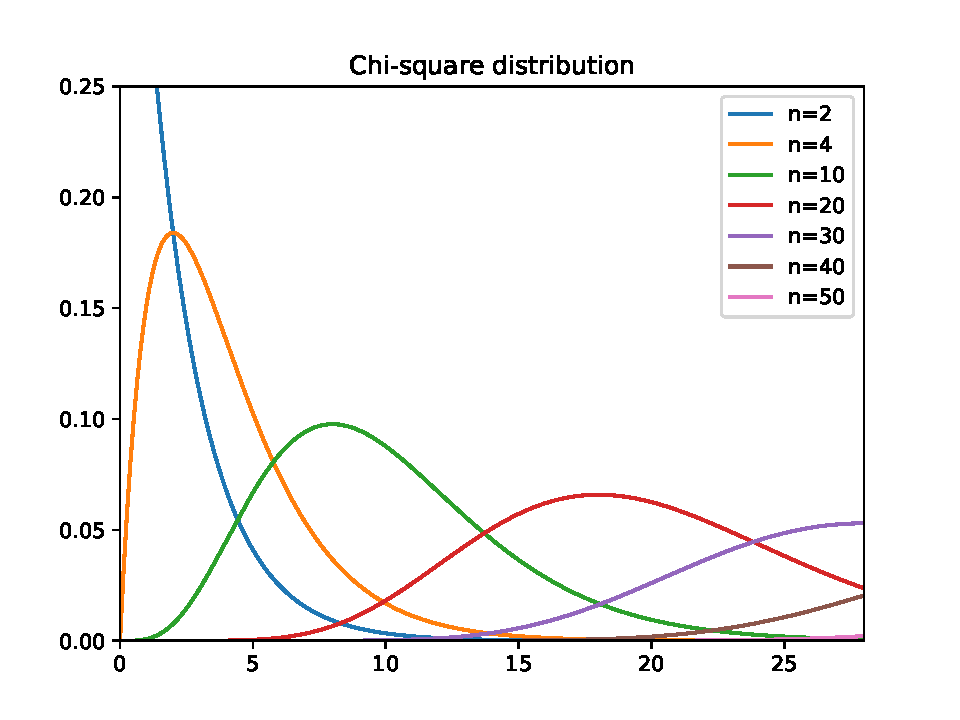
\includegraphics[scale=0.5]{python/ChiSquareDistribution.pdf}
  \caption{$\chi^2$の確率分布。$chi^2$が大きくなるに従って、関数の形が右へシフトしていく。}
\end{figure}


\section{ガウス検定}

検定とは見積もっているパラメーターの真の値について議論する時に用いられる手法である。
例えばガウス分布に従う変数であれば、その真の平均$\mu$と分散$\sigma^2$について知りたいわけである。
しかし実験を何度繰り返しても真の値は絶対に知り得ないわけであるので、実験データから何かを結論づける必要がでてくる。

そこでまず、ガウス分布に従う母集団から無作為に$n$サンプル取り出す試行を考える。
実験データは$\bm{x}={x_1,x_2,...,x_n}$であり、真の値$\mu$と$\sigma^2$を用いると次式の様に標準化できる:
\begin{equation} 
  Z = \frac{x-\mu}{\sigma}
\end{equation}
$Z$は$\mathcal{N}(0,1)$に従う確率変数である。

$Z$はガウス分布に従って様々な値をとるわけであるが、95\%の確率で$[-1.96, 1.96]$の区間に入ることになる。
残り5\%の確率でこの範囲外の値も取り得るが、ほぼ起こらない、と考えてもよい。
以上の議論を少しまとめると、次の様に言い換えることができる。
\begin{itemize}
  \item 「$Z$は$[-1.96, 1.96]$の範囲の値を取る」という条件は95\%の確率で成立する。
\end{itemize}
つまり大体$Z$はこの範囲に存在していると言えるわけである。
ここで、もし仮に$\sigma$が既知であれば、さらに次のように言い換えることができる。
\begin{itemize}
  \item 「$\mu$は$[x-1.96\sigma, x+1.96\sigma]$の範囲の値を取る」という条件は95\%の確率で成立する。
\end{itemize}
ここまできて初めて、真の値$\mu$に対しての条件を引き出せたことになる。

しかし、気をつけなければならないのは、母集団の真の値は大抵全く分からないということである。
上記のような「母平均は分からないけれど、母分散なら分かるよ」というケースはほぼあり得ないのである。
そこで、$\sigma$を何か別の値で置き換えたい気持ちになるが、適当な置き換えをするとそもそも$Z$が従う確率分布が分からなくなり、
結局どんな条件になるか分からなくなってしまう。
そこで登場するのが次節で議論するスチューデント分布である。
このスチューデント分布は、分散の置き換えの指標を示し、また置き換えた後の$Z$が従う確率分布を記述することができる(=存在区間に対する条件を書き出せる)。


\section{スチューデント検定}

\subsection{検定における確率の解釈}

スチューデント分布の$t$は次のように示される:
\begin{equation}
  t = \frac{\hat{x}-\mu}{\sqrt{\frac{s^2}{n}}}
\end{equation}
ここで$\mu$は$x$の母集団の平均、$s$は不偏分散($\sigma$ではない)である。
この関係式を用いることで母平均に対しての条件を考えることができる、というのがスチューデント検定の概要である。
このときに、よく考えないと誤った解釈をしてしまう箇所がある。

$t$が$1-\alpha$の確率で含まれる区間を$[a, b]$で定義する。
確率変数は$t$(正確には$t$の中の$x$)であることに留意すると、次の言い換えが成り立つことが分かる。
$a<t<b$は95\%の確率で成り立つ。

しかし、確率変数は$t$であり、区間$[a,b]$は確率変数でないので、次の言い換えは成り立たないことが分かる。
「$[a,b]$は95\%の確率で$t$を含む」区間は定数であるので、実際の観測値$t$を含むかどうかは確率ではなく「含むor含まない」の2択でしかない。
ここで気をつけなければならないのは、いま着目している確率変数が何か、である。

スチューデント検定では、次のような不等式変形を行う。

\begin{eqnarray}
  a < t = \frac{\hat{x}-\mu}{\sqrt{\frac{s^2}{n}}} < b \\
  \hat{x} - b \sqrt{\frac{s^2}{n}} < \mu < \hat{x} - a \sqrt{\frac{s^2}{n}}
\end{eqnarray}

そのため、次のような誤った解釈が頭に浮かぶ。
「$\mu$は95\%の確率で、区間$[\hat{x} - b \sqrt{\frac{s^2}{n}}, \hat{x} - a \sqrt{\frac{s^2}{n}}]$に含まれる」。しかし、先程の留意事項を思い出せば、
母平均$\mu$は確率変数ではなく、ある決まった(と言っても未知ではあるが)値の定数である。
そのためこの文言は成り立たない。
確率変数はどこまで行っても$t$もしくは$\hat{x}$であるので、正しくは、
「区間$[\hat{x} - b \sqrt{\frac{s^2}{n}}, \hat{x} - a \sqrt{\frac{s^2}{n}}]$は95\%の確率で母平均$\mu$」を含む。である。











